\projecthead{03}{Vibration isolation}{Crystal oscillator mounting study}{Summer internship, 2026}
\textit{Engineering study}
\par\medskip A modal study of a 10 MHz crystal oscillator on four isolators, identifying the frequency ranges where its mounts amplify or reduce vibration.
\par\smallskip {\small\color{muted} Tools: Ansys Mechanical, modal analysis}
\medskip
\noindent
\begin{minipage}[t]{.48\linewidth}\centering\vspace{0pt}
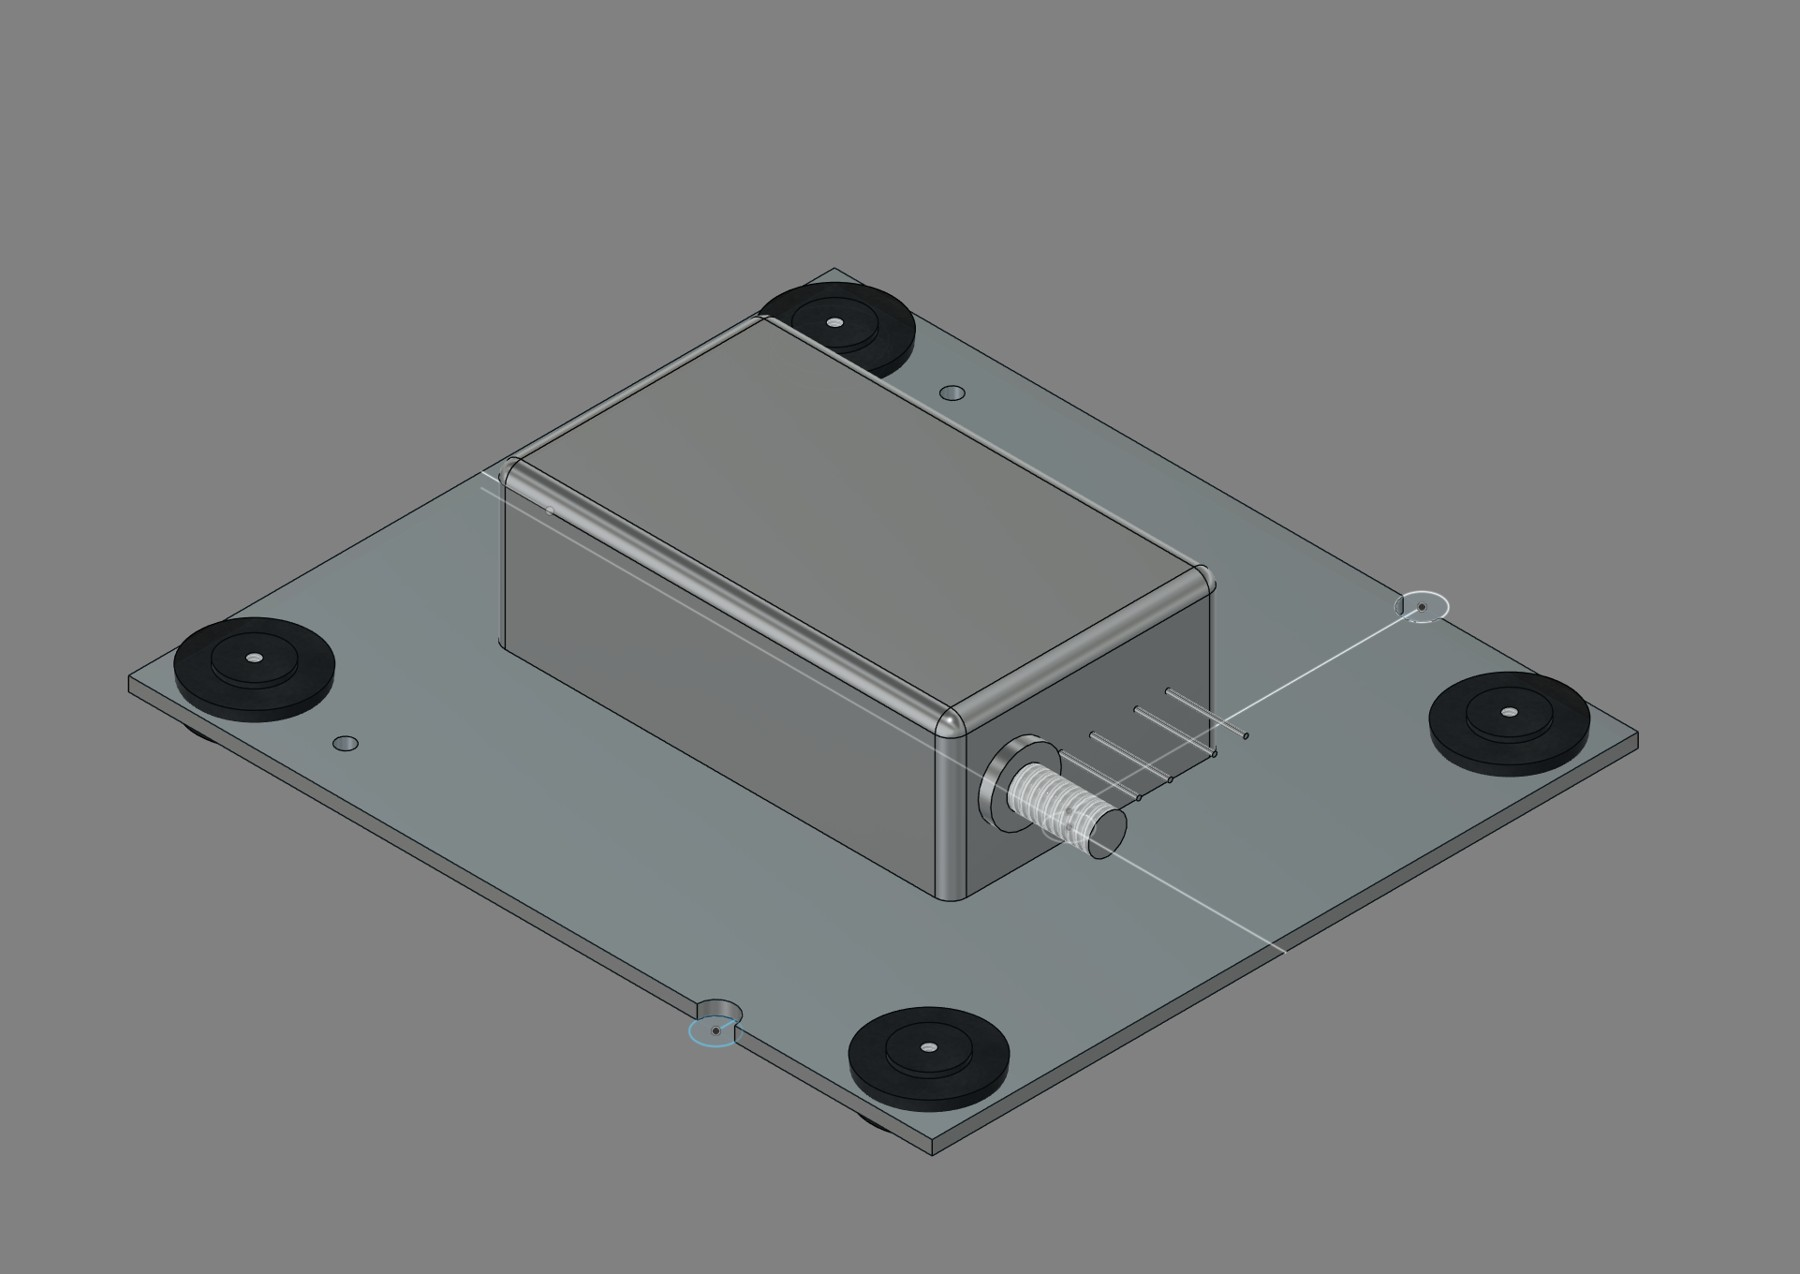
\includegraphics[width=\linewidth,height=2.5in,keepaspectratio]{images/vibration/isolator-assembly.jpg}
\par\smallskip{\footnotesize\color{muted} Oscillator plate and four isolators.}\end{minipage}\hfill
\begin{minipage}[t]{.48\linewidth}\centering\vspace{0pt}
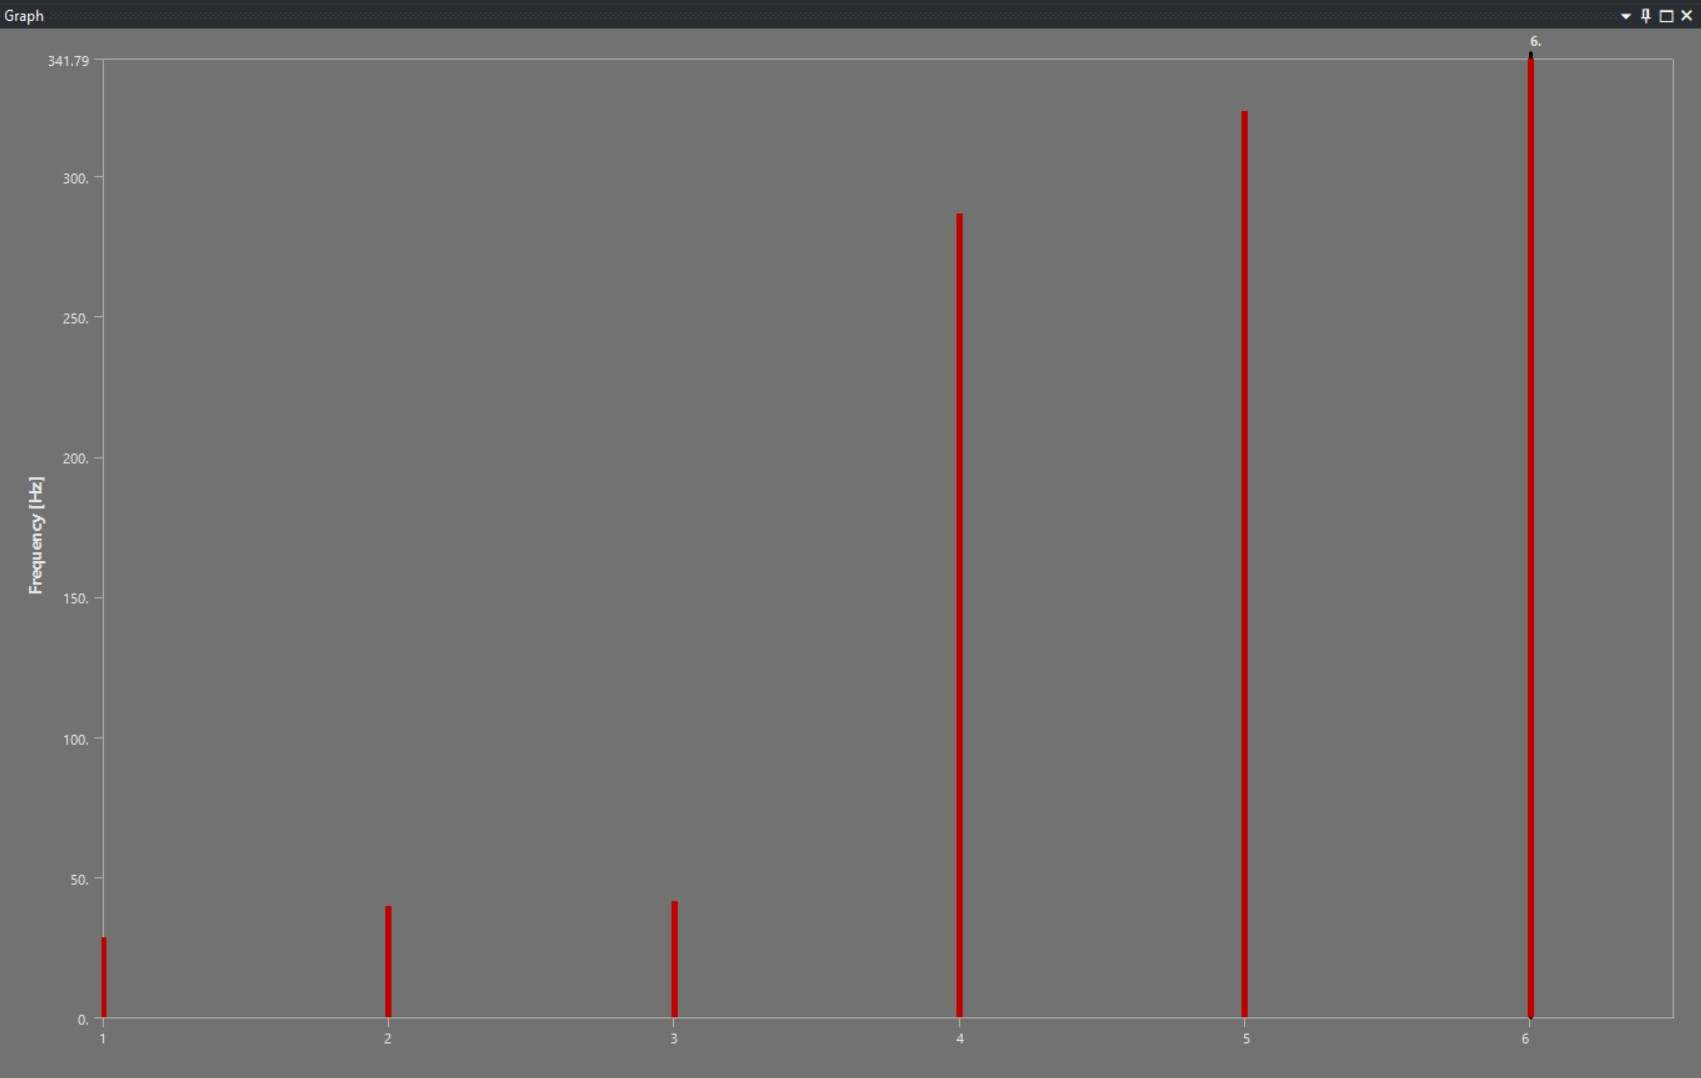
\includegraphics[width=\linewidth,height=2.5in,keepaspectratio]{images/vibration/modal-results.jpg}
\par\smallskip{\footnotesize\color{muted} Ansys results for modes 1-6.}\end{minipage}\hfill
\par\medskip
\subsection*{The assembly}
At East End Assemblies, I studied a Wenzel 501-27521-11 oscillator mounted on a plate with four J-3112-2 isolators.
\subsection*{The analysis}
I ran modal analysis in Ansys Mechanical and examined the first six natural frequencies. Low modes were near 30-50 Hz, where bench motion can be amplified. Isolation began to help above roughly 70 Hz; the mounts stiffened at higher frequencies.
\subsection*{Engineering purpose}
The study described where the mounting system helps and where it does not before installation. These findings apply to the studied assembly and model.